% Template adapted from the Eurographics SGP 2016 template

\documentclass{6838publ}
\usepackage{6838}

\SpecialIssuePaper
\electronicVersion 
\ifpdf \usepackage[pdftex]{graphicx} \pdfcompresslevel=9
\else \usepackage[dvips]{graphicx} \fi

\PrintedOrElectronic

\usepackage{t1enc,dfadobe}
\usepackage{egweblnk}
\usepackage{cite}
\usepackage{lipsum}
\usepackage{amsmath}
\usepackage{amsfonts}


\title[Linear Reconstruction and Material Mapping]{Surface Deformation
  By Linear Reconstruction and Material Mapping}
\author{Hanjun Li\ \ \\
  h1212@mit.edu
}

\begin{document}

\teaser{
 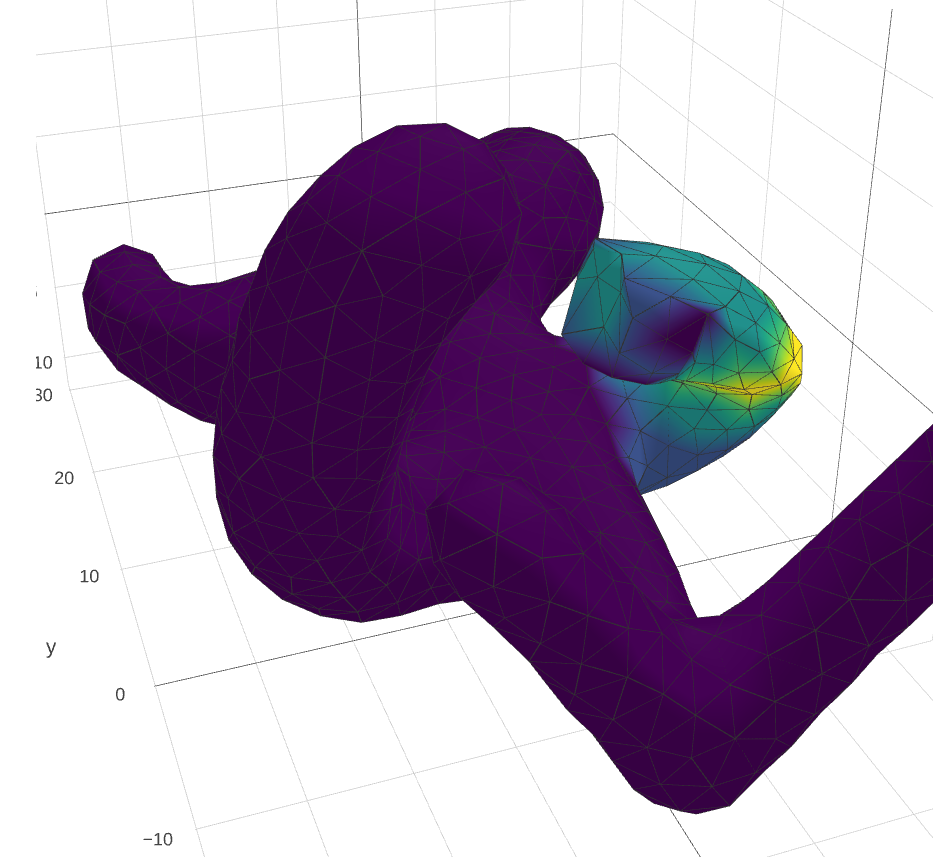
\includegraphics[width=.5\linewidth]{n70soft}
 \centering
  \caption{A folded arm by mapping ``soft'' material to the elbow.}
\label{fig:teaser}
}

\maketitle

\begin{abstract} Linear methods produces fast and usually results for
shape deformation tasks. In this paper, we implement the linear
reconstruction technique proposed in~\cite{wang2012linear}, and apply
it to shape deformation tasks. As a linear algorithm, it fits the
family of linear methods for shape deformation. We also propose a
natural extension to the method to produce more flexible and natural
looking deformation results by applying an additional per-edge material
mapping. By specifying a material mapping, users can customize the
deformation results by including non-geometric information to the
deformation process.
\end{abstract}

\section{Introduction} \label{sec:intro} Surface deformation is a very
common task for artists in many areas, such as computer graphics,
animation, and architectural design. To aid the design process of the
artists, it is therefore desirable to produce interactive response to
user inputs. As the traditional non-linear methods for shape
deformation are too computationally expensive for such objectives,
linear approximation methods become more and more popular. This paper
adopts one novel method for linearly reconstructing surfaces proposed
by~\cite{wang2012linear}, and applies it to surface deformation
tasks. We also propose a natural extension to the algorithm to produce
more flexible and natural looking deformation results. By applying a
per-edge material mapping, users can specify the stiffness of
different areas of a surface, and incorporate this non-geometric
information into the deformation process.

\section{Related Work} \label{sec:related_work} Surface deformation
methods can be generally classified in to non-linear linear
algorithms. While non-linear algorithms usually produce robust and
natural looking results, they are also very computationally
expensive. Linear methods perform well in many cases, but also causes
unnatural looking artifacts in other cases.  ~\cite{botsch2008linear}
provides a comprehensive survey of current linear methods. Since the
method this paper focus on fits into the family of differential
representation methods, we only discuss related methods in this
category. As described in~\cite{botsch2008linear}, there have been
many proposed differential representations of surfaces, including
gradient, laplacian, and local frame coordinates. In the discrete
setting, all of those representations result in values stored on each
face or edge of the surfaces. A naive approach would be to directly
minimize the differences of those differential representations between
the original surface $S$, and the deformed surface $S'$.
\begin{equation} \label{eq:naive_energy} \min_{p'} \sum_{i} A_{i} ||
D(p'_{i}) - D(p_{i})||
\end{equation} Where $p, p'$ are vertices of the original and deformed
surfaces, and $D()$ is the differential operator considered by
different methods.  However, such an optimization doesn't necessarily
minimize the differences between $s$, and $s'$, because each
differential value, either on an edge, or on a face is relative to a
local frame. Minimizing Eq. \ref{eq:naive_energy} only make sense when
the local frames are aligned between the surfaces.
\par To determine the transforms on each local frame, many methods
have been proposed. By requiring users to input a local transform
along with a set of constraint points, $H$, one can interpolate the
transform by a smooth scalar field $s$. Possible definition of the
scalar field $s$ includes the geodesic distance function from $H$, the
harmonic function that satisfies $Ls = 0$, or the result of the
minimization problem $\min_{s} \sum_{j\in N_{1}(v_{i})} \phi_{ij}
||s_{i} - s_{j}||^2$, where $\phi_{ij}$ is a per-edge weight,
connecting face $f_i$ and $f_j$. The last one is called material
mapping because the per-edge weight $\phi_{ij}$ determines the
stiffness of surface by specifying the objective difference of the
between scalar field between adjacent faces $f_{i}$ and $f_{j}$.  If
the difference is small, then the local transform $T_{i}$ and $T_{j}$
are similar, which corresponds to a stiff surface area.  This idea of
using per-edge weight to control the stiffness of surfaces is later
applied to the linear reconstruction method as described in Section
\ref{sec:technical_approach}. After determined a set of local
transform $T_{i}$, one can then minimize the modified version of
Eq. \ref{eq:naive_energy}:
\begin{equation} \min_{p'} \sum_{i} A_{i} || D(p'_{i}) -
T_{i}(D(p_{i}))||
\end{equation}
\par The technique proposed by \cite{wang2012linear} similarly
considers a differential representation of surfaces, but it solves for
the local transforms $T_{i}$ implicitly by proposing a discrete
version of the fundamental theorem of surfaces, which combines and
solves for (transformed) local frames and local coordinates together
in a natural way.

\section{Technical Approach}\label{sec:technical_approach} To
implement the proposed method of \cite{wang2012linear}, we first need
to understand the proposed discrete theorem of surfaces. In plain
words, the theorem says that given the connectivity of a set of
triangles, the edge lengths, as the discrete first fundamental form,
and the dihedral angles between adjacent triangles, as the discrete
second fundamental form, we can uniquely determine a surface mesh, up
to translation and rotation. The theorem can be illustrated and
understood by the following steps to reconstruct the surface.
\begin{enumerate}
\item First, we can use the law of cosines to compute the inner angles
of each triangle face of the surface, from its edge lengths.
\item Second, we can assume a local frame $f_{i} = (e_{i1}, e_{i2},
e_{i3})$ of each triangle by using the normalized first edge as $e_1$,
the face normal as $e_3$, and $e_3 \times e_1$ as $e_2$. The first
edge can be consistently determined by the triangle connectivity
data. (i.e. use the first vertex to second vertex of each triangle as
the first edge.) Although we don't have a concrete description of each
local frame, we can compute the coordinate of the edge vectors with
respect to each local frame. (The first edge always has $(edge\_len,
0, 0)$ as its coordinate. The coordinates of the other 2 edges can be
calculated as cosine and sine of the inner angles computed in step
one.)
\item Third, we can calculate the rotation matrices $R_{ij}$ that
transform one local frame $f_{i}$ to the ones of its adjacent
triangles $f_{j}$, as a product of three rotations. The leftmost
rotation rotates the local frame $f_{i}$ of triangle $i$ around
$e_{i3}$, the normal direction, so that $e_{i1}$ aligns with the edge
$E_{ij}$ it shares with triangle $f_{j}$. The middle rotation rotate
the frame around $e_{i1}$, now aligned with the shared edge, so that
$e_{i3}$ aligns with the normal direction of triangle $j$. The right
most rotation rotate the frame around $e_{i3}$ axis, now aligned with
the normal of $j$, so that the frame aligns with the local frame of
triangle $j$, $f_{j}$.
\item Finally, fixing any orthonormal basis for one triangle, and a
position for one of its vertex, we can construct the whole
surface. The other 2 vertices are determined by their coordinates and
the fixed local frame. We can further determine the local frames for
the adjacent faces using the rotation matrices, and then, their
vertices.
\end{enumerate} Therefore, the discrete fundamental forms, the edges
and dihedral angles determines a surface, as stated in the theorem.
\par We can then implement the algorithm to linearly reconstruct a
surface from its discrete first and second fundamental
forms. According to the above steps, it's clear that for a consistent
surface, we have the following frame equation:
\begin{equation}\label{eq:frame_equation} \forall e_{ij} \in E, f_{j}
= f_{i} R_{ij}
\end{equation} An illustration of the frame equation is shown in
Figure \ref{fig:frame_equation}.
\begin{figure}[t!]  \centering
  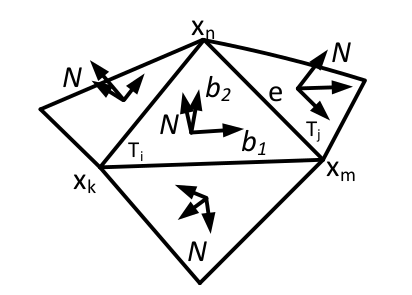
\includegraphics[width=.6\linewidth]{frame_equation}
  \caption{ This figure illustrate the frame equation,
Eq. \ref{eq:frame_equation}.  We can see the to transform the frame
$f_{i} = (b_{i1}, b_{i2}, N_{i})$ to align with $f_{j}$, we first
rotate it along $N_{i}$ to align $b_{i1}$ with edge $mn$. Then, we
rotate it along the new $b_{i1}$ vector, so that $N_{i}$ aligns with
$N_{j}$.  We finally rotate it along the new $N_{i} = N{j}$ so that
$b_{i1}$ is aligned with $b_{j1}$}.
  \label{fig:frame_equation}
\end{figure} We similarly have the the following edge equations: (for
any triangle $T$ containing vertex $n$ and $m$)
\begin{equation}\label{eq:edge_equation} x_{n} - x_{m} = (a^{1}_{mn,
T} e_{1,T} + a^{2}_{mn, T} e_{2,T})
\end{equation} Where $a$ are the edge coordinates in the local frame
of $T$. An illustration
\begin{figure}[t!]  \centering
  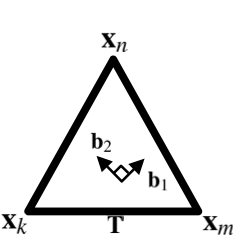
\includegraphics[width=.6\linewidth]{edge_equation}
  \caption{ This figure illustrate the edge equation,
Eq. \ref{eq:edge_equation}.  We can see that vector $Xn - Xm = E_{mn}$
is determined by 2 coefficients with respect to the local frame
$(b_{2}, b_{1}, (N))$}.
  \label{fig:edge_equation}
\end{figure} of the edge equation is shown in Figure
\ref{fig:edge_equation}. After following the above described steps to
calculate the rotations matrices $R_{ij}$ and local edge coordinates
$a^{1}, a^{2}$, we can solve Eq. \ref{eq:frame_equation} and
Eq. \ref{eq:edge_equation} by minimizing the following energy term:
\begin{equation} \label{eq:frame_energy} E_f(\mathbf{f}) = \frac{1}{2}
\sum_{e \in E, e = T_i \cap T_j} w_e^{-1} || f_j - f_iR_{ij} ||^2
\end{equation}
\begin{equation} \label{eq:edge_energy} E_x(\mathbf{x}, \mathbf{f}) =
\frac{1}{2} \sum_{e=v_mV_n} \sum_{T \ni e} w_{e, T} ||x_n - x_m -
f_T(a^1_{e,T}, a^2_{e,T}, 0)^T ||^2
\end{equation}
\begin{equation} \label{eq:sum_energy} E_M(\mathbf{x}, \mathbf{f}) = w
E_f + E_x
\end{equation} Where $E_f$ corresponds to Eq. \ref{eq:frame_equation},
and $E_x$ corresponds to Eq. \ref{eq:edge_equation}. $w_{e}$ in the
equations are the cotangent edge weights, given by:
\[w_{mn} = \cot(\alpha_{mn}) + \cot(\beta_{mn})
\] where $\alpha_{mn}$ and $\beta_{mn}$ are the angles opposite to
edge $mn$.
\par To minimize the energy terms, we first, rewrite the energy
equations with corresponding matrix representations:
\[E_f = \frac{1}{2} ||W_f^{1/2} R_3 \mathbf{f'}||^2\]
\[E_x = \frac{1}{2} ||W_{x,l}^{1/2} (R_1 \mathbf{x} - R_{2, l}
\mathbf{f'}) ||^2 + \frac{1}{2} ||W_{x,r}^{1/2} (R_1 \mathbf{x} -
R_{2, r} \mathbf{f'}) ||^2\] Where $W$ is the cotangent weight matrix,
$R_{1}, R_{2}, R_{3}$ are calculated according to the corresponding
definitions of $E_{f}$ and $E_{x}$. Note that since $E_{x}$ counts the
two triangles connected by every edge, we separate it into two
equations, with $W_{l}, M_{2,l}$ corresponds to the triangles on the
left hand side of every edge. Now, we can derive and solve the
following linear systems:
\begin{equation*}
\begin{split} (wR_3^T W_f R_3 - R_{2, l}^T W_{x, l} R_{2, l} - R_{2,
r}^T W_{x, r} R_{2, r})\mathbf{f'} + \\ (R_{2, l}^T W_{x, l} R_1 +
R_{2, r}^T W_{x, r} R_1)\mathbf{x} = 0
\end{split}
\end{equation*}
\[( - R_1^T W_{x, l} R_{2, l} - R_1^T W_{x, r} R_{2, r})\mathbf{f'} +
(R_1^T W_{x, l} R_1 + R_1^T W_{x, r} R_1)\mathbf{x} = 0\] This sparse
linear equation can be solved with a seed vertex position that
specifies the translation of the surface, and a seed local frame that
specifies the rotation. Figure \ref{fig:rotated} shows an example of
first building the fundamental form representation of a surface, and
then solve the system with an arbitrary set of seed vertex and frame.
\begin{figure}[t!]  \centering
  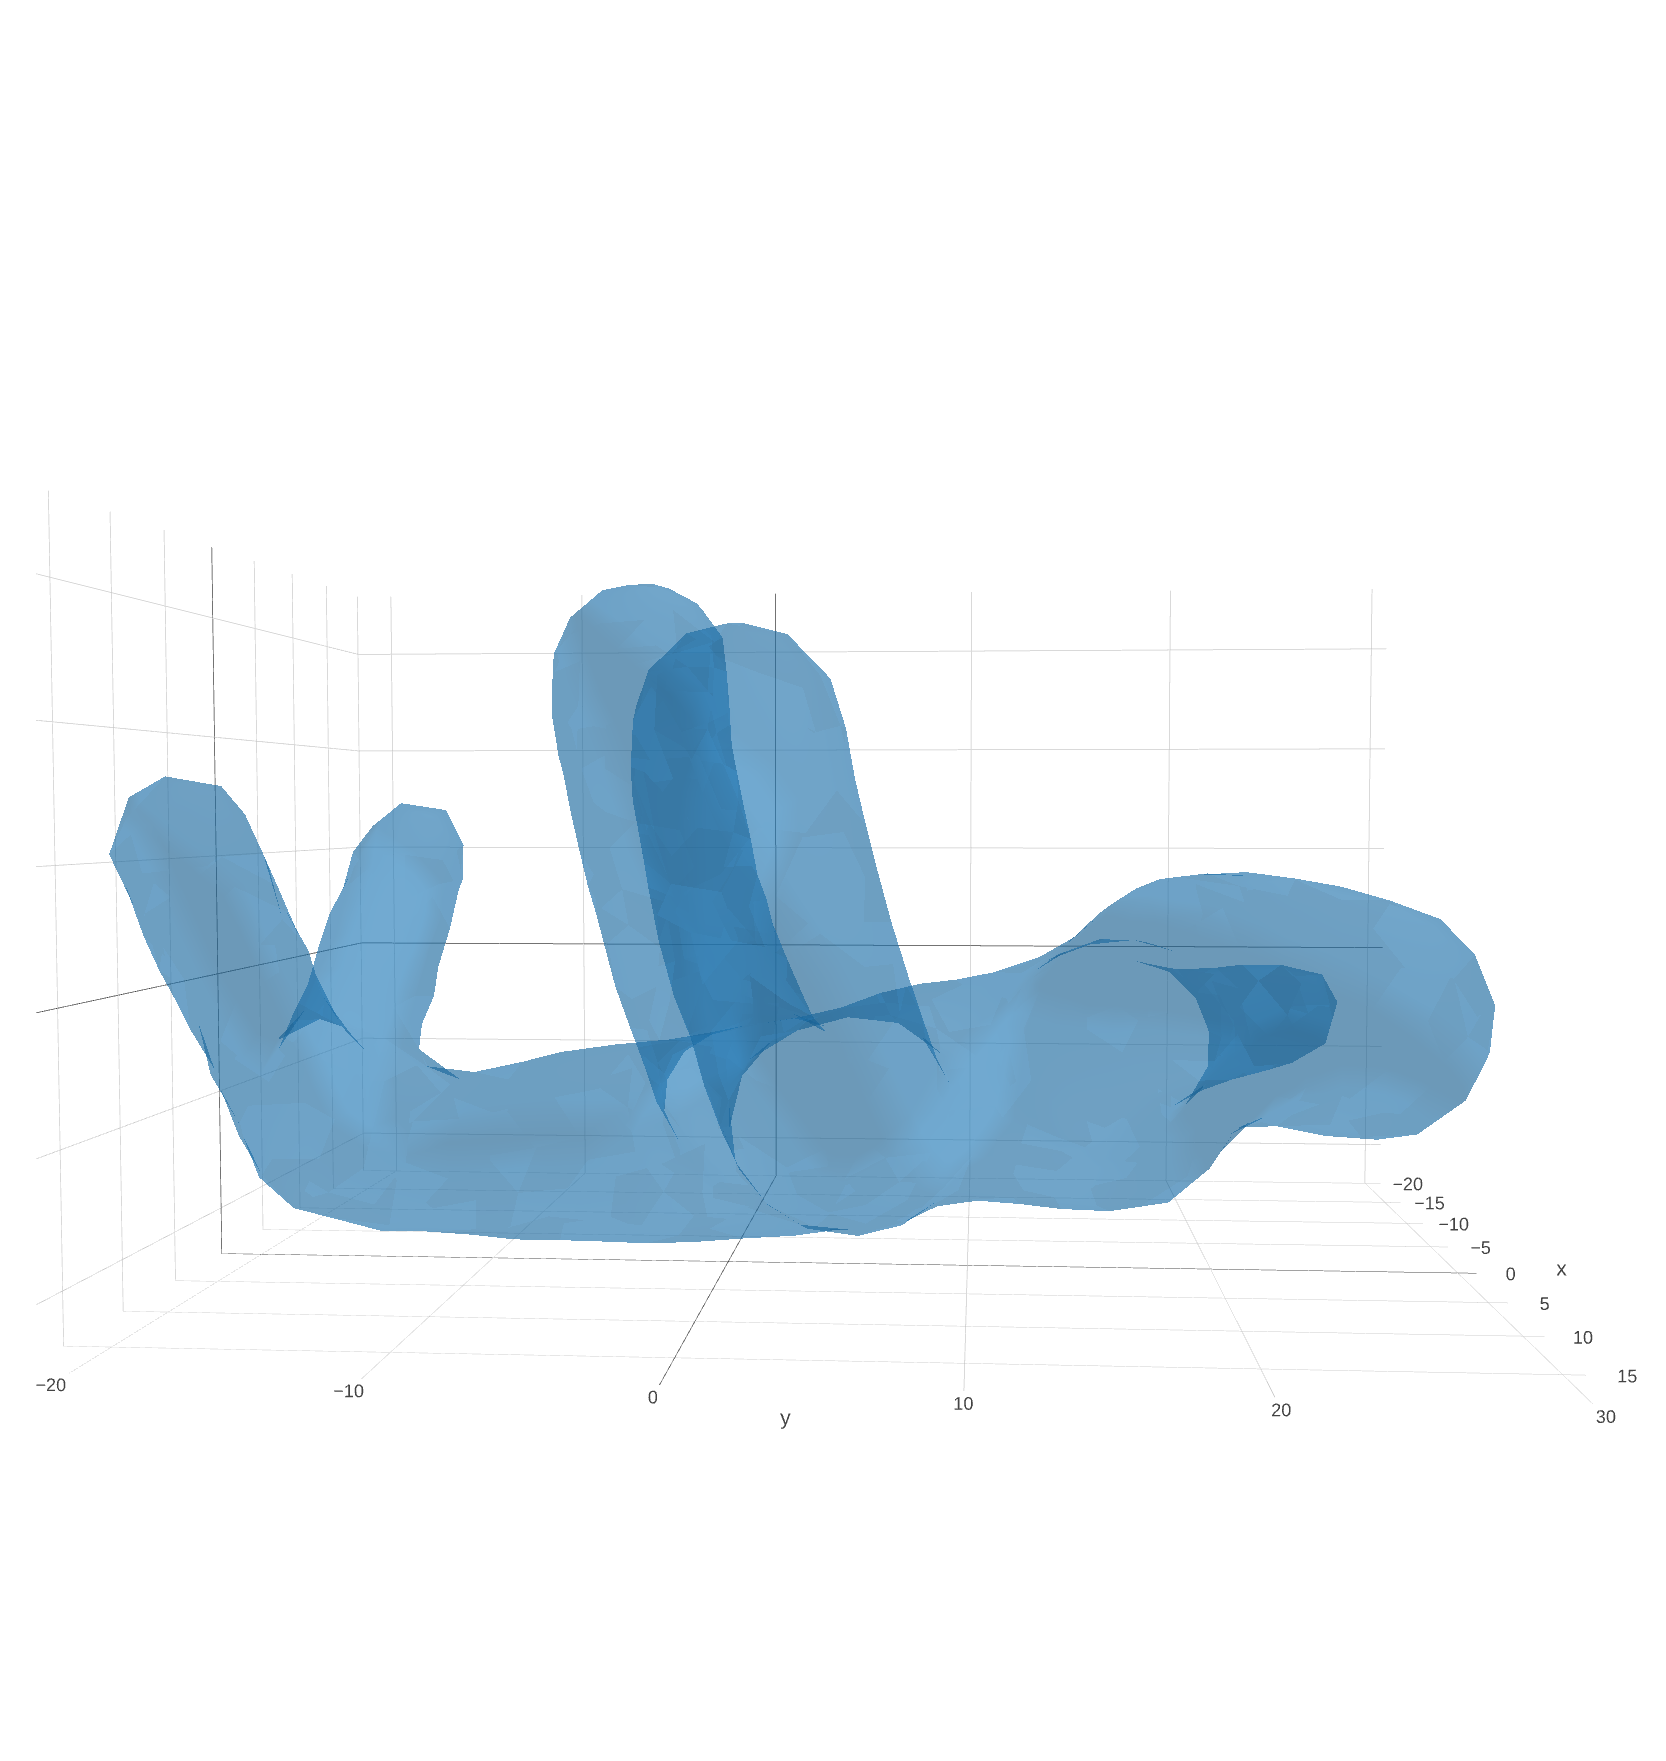
\includegraphics[width=.6\linewidth]{original}
  \caption{The figures are produced using the provided data file for
homework 2. This is a plot for the original mesh data. }
  \label{fig:original}
\end{figure}
\begin{figure}[t!]  \centering
  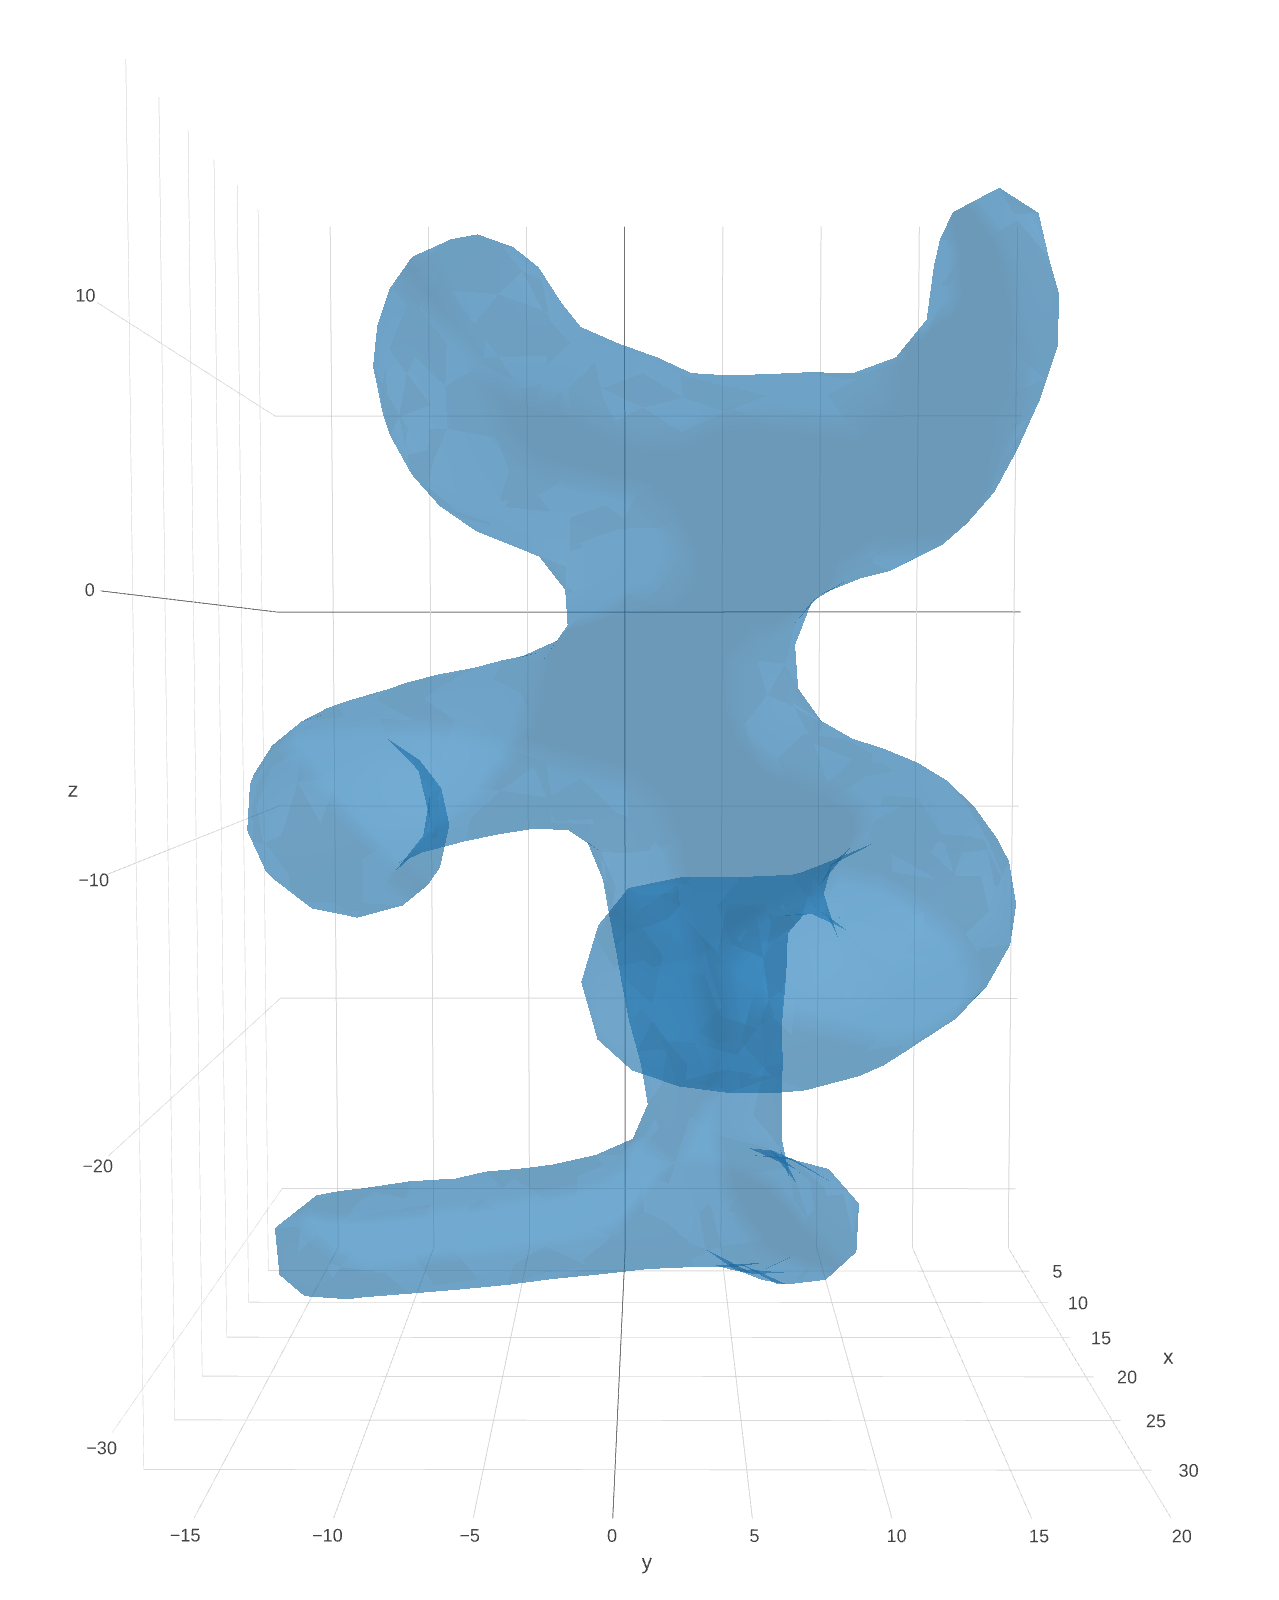
\includegraphics[width=.6\linewidth]{rotated}
\caption{This is the result of solving the linear system derived from
the energy terms in Eq. \ref{eq:sum_energy}, with an arbitrary
$\mathbf{f_0}$ and the original $\mathbf{x_0}$ as the constraint
(seed).  Compare with Figure \ref{fig:original} to see the rotation
and translation effect. This illustrate that the discrete fundamental
form representation of the surface is rigid motion invariant.}
\label{fig:rotated}
\end{figure} In order to apply this reconstruction algorithm to
surface deformation, we first determine a set of vertices as the
handle $H$, and specify their desired positions as hard constraints to
the linear system. Usually, we want to only deform a surface locally
around some interesting features, but any deformation to a local
handle will necessarily affect all other local frames. Therefore, in
addition to the movable handle $H$, we also use a fixed handle $H_{f}$
to fix the areas that we want to keep the surface unchanged. Figure
\ref{fig:original_handle} and Figure \ref{fig:stretched_handle} shows
an example of using movable and fixed handles to stretch an arm of the
figure. The fixed handle is shown in dark purple, while the movable
handle is shown in bright yellow.
\begin{figure}[t!]  \centering
  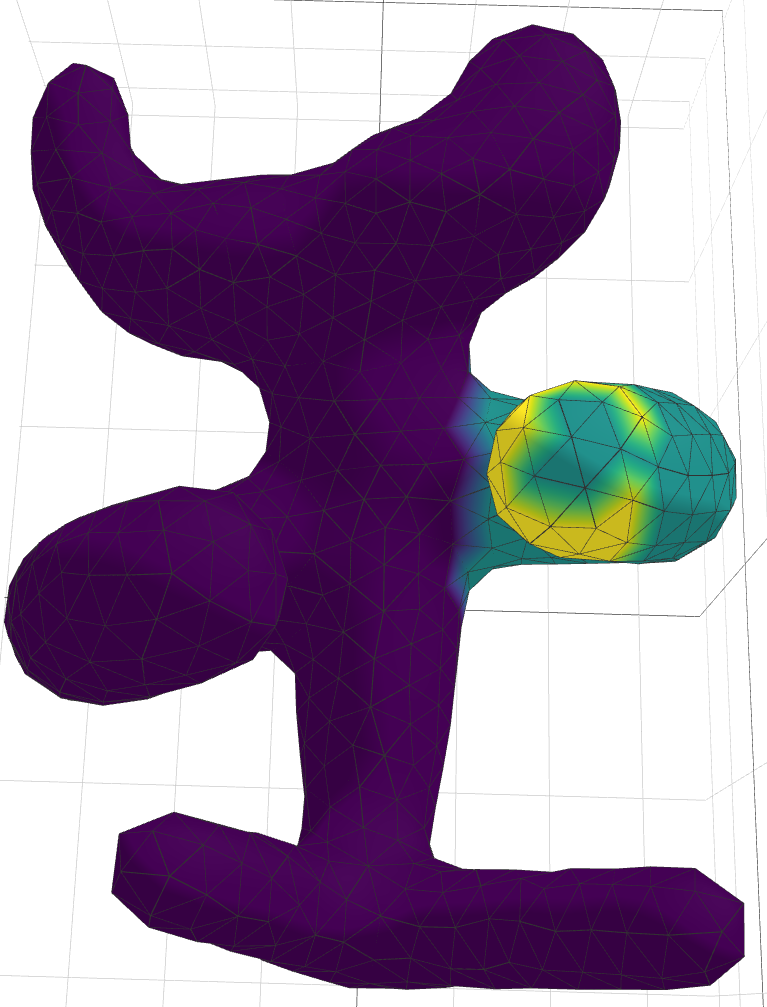
\includegraphics[width=.5\linewidth]{original_handle}
  \caption{The original mesh, with texture color showing the area of
the fixed handle (dark purple), and the area of the movable handle
(bright yellow). }
  \label{fig:original_handle}
\end{figure}
\begin{figure}[t!]  \centering
  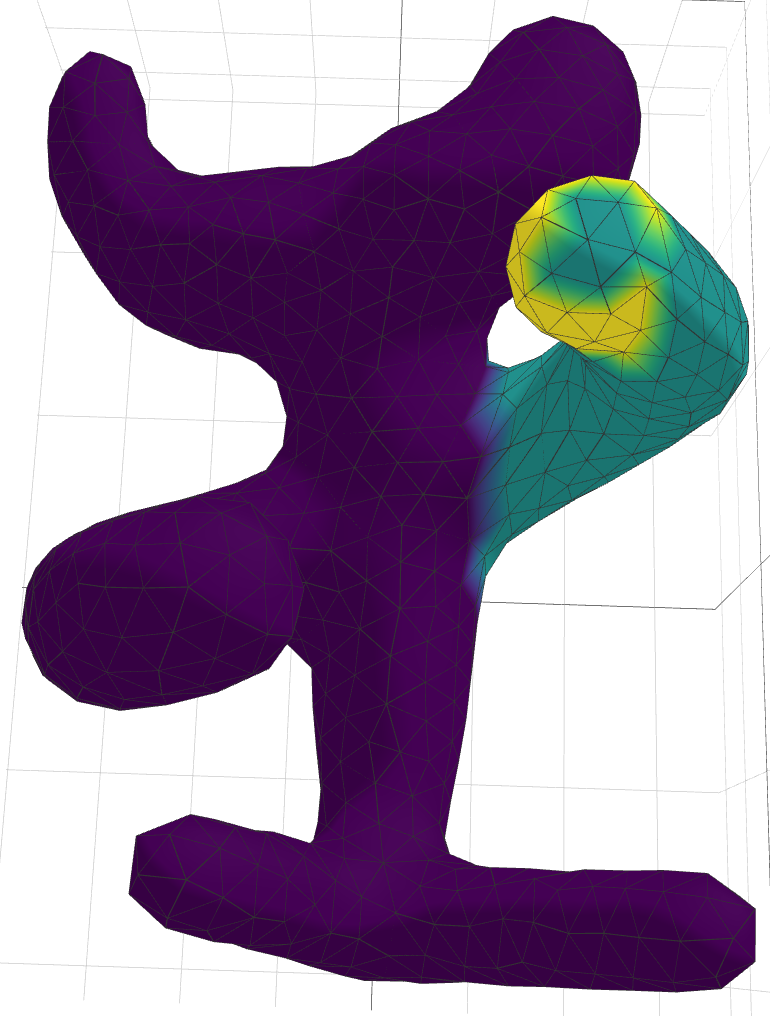
\includegraphics[width=.5\linewidth]{stretched_handle}
\caption{This figure illustrates how to use fixed handle (dark purple
area) and movable handles (bight yellow area) to locally deform a
mesh around interesting feature points (the arm).  Compare with Figure
\ref{fig:original_handle} to see the deformed arm.}
    \label{fig:stretched_handle}
\end{figure} Although the shape deformation methods tries to produce
natural looking surface deformations, sometimes the expected natural
ways of deformation cannot be inferred solely from the geometry of the
surface. For example, we may naturally view the deformed part in
Figure \ref{fig:stretched_handle} as something similar to human
arms. That is, if we fold the ``arm'' inwards, we expect to see it
bending more in the inner center area corresponding to human
elbows. However, from the geometric point of view, there is no obvious
clue that a cylinder looking surface should bend non-uniformly in
certain areas. To make our deformation algorithm more flexible, we
include this non geometric information by adding a material mapping to
the surface, and incorporate it into the algorithm.
\par Note that in Eq. \ref{eq:frame_energy} and
Eq. \ref{eq:edge_energy}, $E_{f}$ and $E_{x}$ already include a
cotangent edge weight $w_{e}$. We can naturally add our material
related information into the energy by multiplying the edge weights
with a per-edge scalar that accounts for the desired material
properties. Intuitively, $E_{f}$ tries to minimize the difference of
cross edge rotation matrices $R_{ij}$ between a deformed surface and
the original surface. Since $R_{ij}$ is determined by the dihedral
angles of the surface, $E_{f}$ corresponds to minimizing the bending
of the deformed surface. Similarly, since $E_{x}$ tries to minimized
the difference of the local coordinates of every edge, it corresponds
to minimizing the stretching of the deformed surface. Therefore, to
make a certain area easier to fold, we can put a higher weight for the
(approximately) bending energy $E_{f}$ and a lower weight for the
(approximately) stretching energy $E_{x}$ for the corresponding
edges. The low weight for $E_{x}$ makes shrinking the area easy, while
the higher weight for $E_{f}$ enforces the curvature of the shrink
area.
\par To implement this idea, we need a smooth material mapping that
satisfies the required material property. Ideally, we would want some
automated method that interpolates a smooth function on the surface
requiring minimum user input. We can solve the harmonic function that
is similar to the harmonic interpolation technique described in
Section \ref{sec:related_work}.  However, due to the time constraint,
in the experiment of this project, we manually assign a approximately
smooth weight mapping on to the desired area by searching vertex
positions for target areas. Continuing with the arm deformation
example shown in Figure \ref{fig:n50soft}, Figure \ref{fig:n70soft}
and Figure \ref{fig:n70rigid}, we map a soft material (i.e. easy to
fold) to the elbow looking area (shown in bright yellow), and then
fold the arm inward using the above described algorithm with a fixed
handle (shown in dark purple) and a movable handle (shown also in dark
purple, around the fist area of the deformed arm).
\begin{figure}[t!]  \centering
  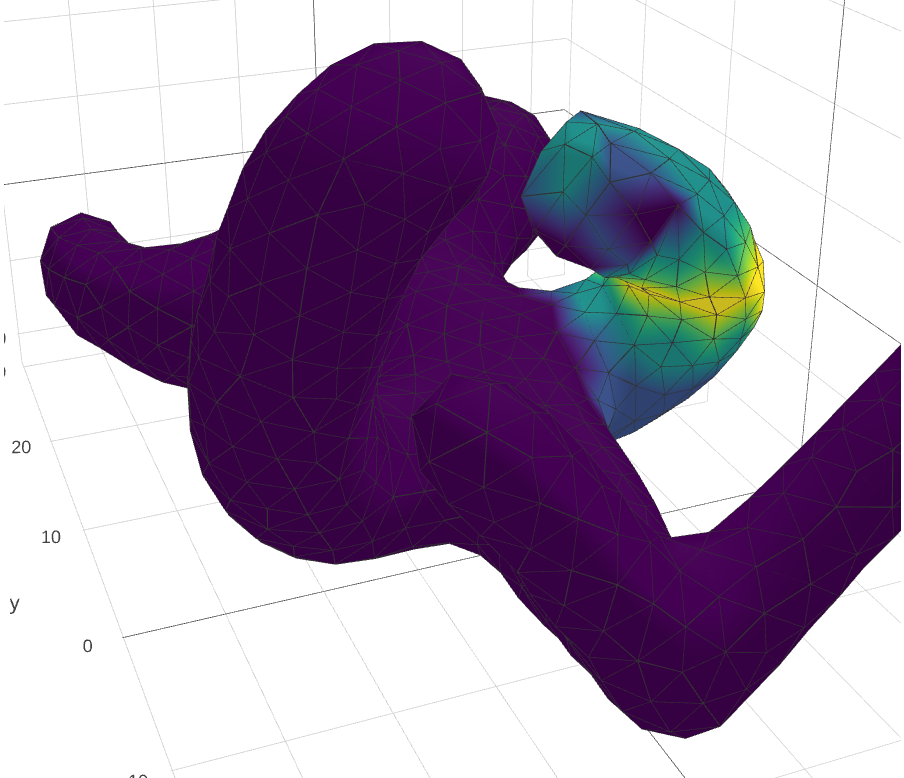
\includegraphics[width=.6\linewidth]{n50soft}
  \caption{The folded arm with material mapping.  This figure
illustrates the effect of applying the material mapping to the target
area, to model a easier to fold surface area that is similar to a
human elbow. The dark purple areas are the fixed and movable handle
points, while the softness of the surface is color coded, with the
bright yellow area being the softest. }
  \label{fig:n50soft}
\end{figure}
\begin{figure}[t!]  \centering
  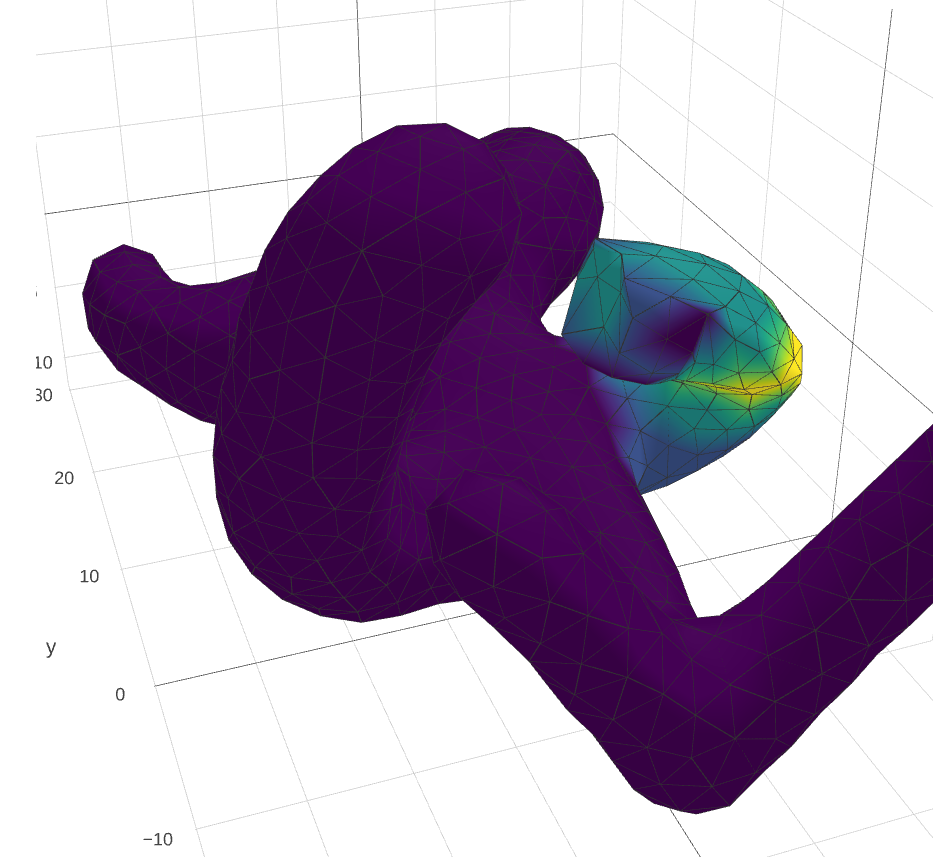
\includegraphics[width=.6\linewidth]{n70soft}
  \caption{The more folded arm with material mapping.  This figure
shows a more extreme example of folded arm. We can compare this with
Figure \ref{fig:n50soft} to see how the surface deform after material
mapping. We can also compare with Figure \ref{fig:n70rigid} to see
that with material mapping, the deformed surface looks more natural
and has less distortion.}
  \label{fig:n70soft}
\end{figure}
\begin{figure}[t!]  \centering
  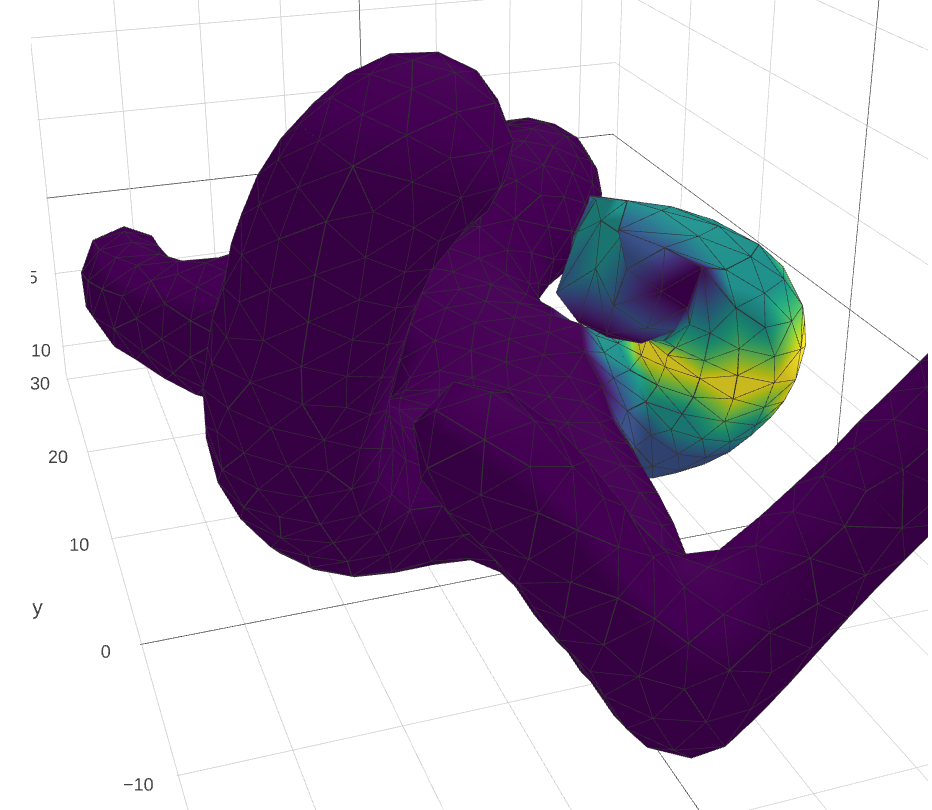
\includegraphics[width=.6\linewidth]{n70rigid}
\caption{The more folded arm without material mapping.  We can observe
a apparent distortion to the arm when it's deformed using the original
algorithm, trying to preserve the edge lengths by widening the arm,
while the algorithm that incorporates the material mapping avoids the
unnatural widening, as shown in Figure \ref{fig:n70soft}}
  \label{fig:n70rigid}
\end{figure} Comparing Figure \ref{fig:n70soft} and
\ref{fig:n70rigid}, we can see that the original algorithm produces
unnatural widening of the arm area in an effort of trying to preserve
edge lengths of compressed area. With material mapping applied, the
algorithm let the inner elbow area naturally shrink, and produces a
more natural looking folded arm.
\par Note that during experiment, it's observed that the algorithm
requires the mapping to be smooth. If we apply a naive mapping like a
step function, with lower weights in the elbow area, we would get
highly discontinuous deformation shown in
\ref{fig:step_mapping}. Also, the relative weights to put on the areas
also need careful calibration. It took several tries to get the
good looking results shown in Figure \ref{fig:n50soft} and Figure
\ref{fig:n70soft}, while a bad choice of weight, (e.g. too low)
produces results shown in \ref{fig:low_weight}.
\begin{figure}[t!]  \centering
  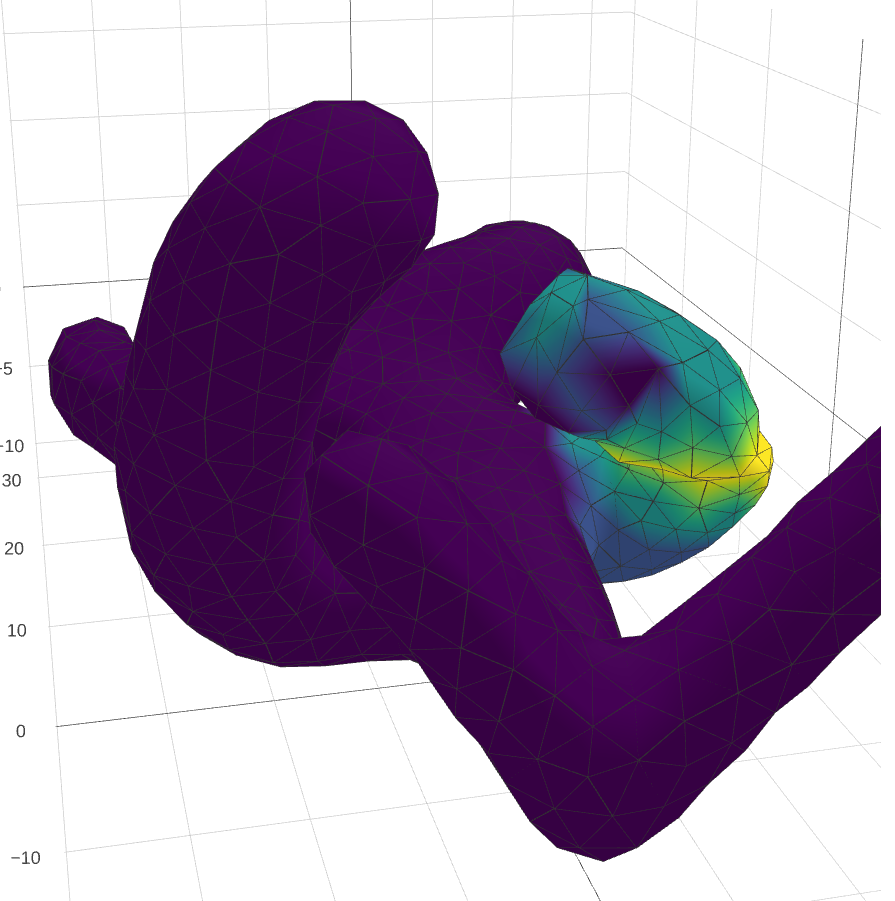
\includegraphics[width=.6\linewidth]{discontinuous}
  \caption{The more folded arm using a not smooth material mapping. On
the boundary of the soft material and the normal material, the
deformed surface shows discontinuity due to large change of dihedral
angle. This deformation uses the same constraint as Figure
\ref{fig:n50soft}}
  \label{fig:step_mapping}
\end{figure}
\begin{figure}[t!]  \centering
  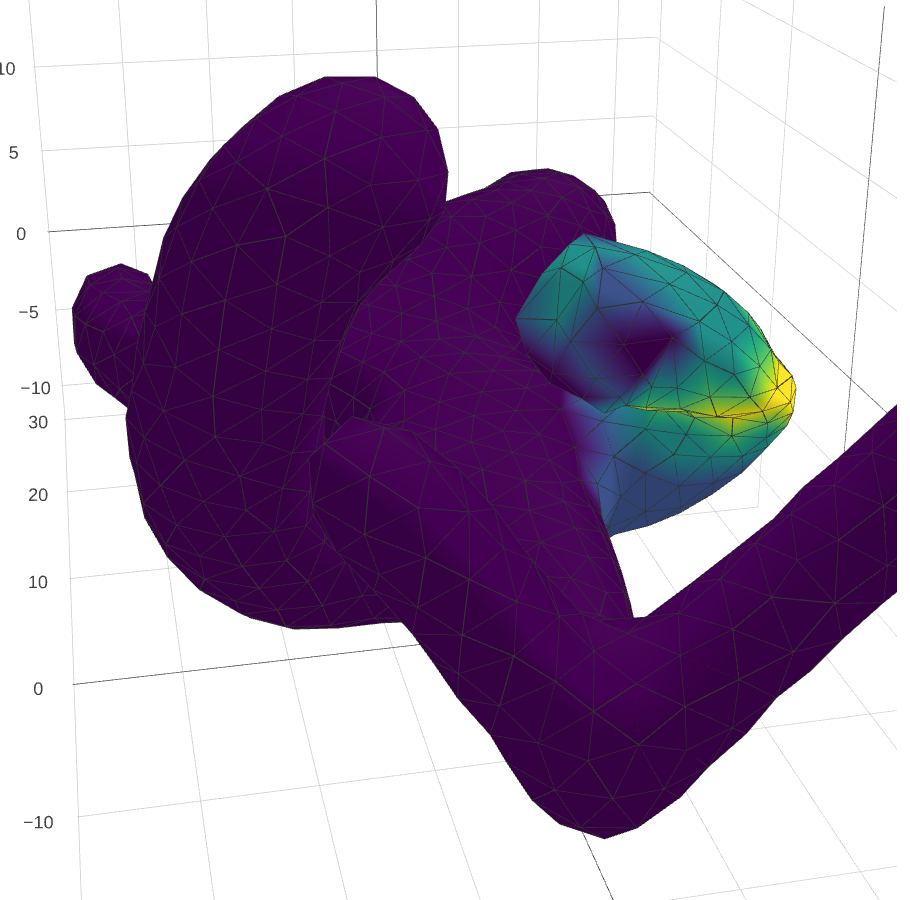
\includegraphics[width=.6\linewidth]{too_soft}
  \caption{The more folded arm using too soft a material. This also
results in unnatural looking deformation. This deformation uses the
same constraint as Figure \ref{fig:n50soft}}
  \label{fig:low_weight}
\end{figure}
\section{Conclusion and Future work} In this paper, we implement the
linear surface reconstruction technique proposed by
\cite{wang2012linear} and apply it the surface deformation tasks. This
method fits in the family of linear deformation algorithm, but has the
advantage of combining the local frame transformation and local
coordinate representation into a single linear optimization
problem. Therefore, this method does not require users to input local
transformations of the handle points, and solve for local
transformations implicitly. We then propose to combine the material
mapping technique for local transformation interpolation with the
linear reconstruction algorithm, by simply multiplying the edge weight
term $w_{e}$ in Eq. \ref{eq:frame_energy} and Eq. \ref{eq:edge_energy}
with a per edge weight that corresponds to a material mapping that
controls the stiffness of surface areas under deformation. This gives
a more flexible and more powerful algorithm that can incorporate
non-geometric details into the deformation process.
\par However, determine the proper material mapping can be
tricky. Firstly, it would ideally be an automated process of
interpolating values according to a few user input points.  We can
treat this as a similar problem to local transformation interpolation,
and apply the harmonic interpolation method. In the future, we can
implement this idea and integrate it into our surface deformation
pipeline. Secondly, the values of the material mapping needs careful
design. This would require a very good understanding of the energy
terms $E_{f}$ and $E_{x}$ defined in Eq. \ref{eq:frame_energy} and
Eq. \ref{eq:edge_energy} from the user. The process of defining a good
material mapping may require many experiments. A good thing is that
once the mapping is determined, it is always valid for the
corresponding surface, before and after deformations.
\bibliographystyle{eg-alpha-doi} \bibliography{6838bibsample}

\end{document}

%%% Local Variables: %%% mode: latex %%% TeX-master: t %%% End:
